% vim: textwidth=110
% Suppress some acceptable compilation warnings
\RequirePackage[save,showerrors]{silence}
\WarningFilter{transparent}
  {Loading aborted} % Used (or at least tried) by the svg package
\WarningFilter{multicol}
  {May not work with the twocolumn option} % I'm not really using the multicol package
\WarningFilter{latex}
  {Marginpar on page} % Margin stuff moved to not overlap with other stuff, this is fine
\WarningFilter{caption}
  {Unknown document class} % the caption package doesn't know about llncs
\WarningFilter{caption}
  {Unused} % the caption package warns on unused setup (here, a captionsetup)

% llncs class documentation:
% https://ctan.tetaneutral.net/macros/latex/contrib/llncs/llncsdoc.pdf
\documentclass[dvipsnames,runningheads]{llncs}

% language settings
\usepackage[main=french,english]{babel}
\newcommand{\en}[1]{\foreignlanguage{english}{\emph{#1}}}
\usepackage{csquotes}
\MakeOuterQuote{"}
% Fix LLNCS language handling of the "keywords" part of the abstracts
\addto{\captionsfrench}{\renewcommand{\keywordname}{\textbf{Mots-clé:}}}
\addto{\captionsfrench}{\renewcommand{\andname}{et}}

% Hyphenation
\hyphenation{Git-Hub}

% links setup
\usepackage[nobiblatex]{xurl}
\usepackage{hyperref}
\hypersetup{colorlinks=true}

% bibliography settings
\usepackage[hyperref=true,isbn=false,eprint=false,giveninits=true]{biblatex}
% redefine the "title" field style to remove quotation marks
\DeclareFieldFormat*{title}{#1}
% redefine the "url" field to remove protocol information (https://)
\DeclareSourcemap{
    \maps[datatype=bibtex]{
        \map{
            \step[fieldsource=url, final=true]
            \step[fieldset=verba, origfieldval, final=true]
            \step[fieldsource=verba, match=\regexp{\A(ht|f)tp(s)?:\/\/}, replace={}]
        }
    }
}
\DeclareFieldFormat{url}{%
    \mkbibacro{URL}\addcolon\space
    \href{#1}{\nolinkurl{\thefield{verba}}}%
}
\DefineBibliographyExtras{french}{\restorecommand\mkbibnamefamily}
\addbibresource{../references.bib}

% Hypotheses
\newtheorem{hypo}{Hypothèse}[theorem]

% For file inclusion and figure formatting
\usepackage{caption}
\usepackage{subcaption}

% Other
\usepackage{todonotes}
\usepackage{mathtools}
\usepackage[inline]{enumitem}

\title{L'Identification des Projets de Logiciel Libre Accessibles aux Nouveaux Contributeurs}
\titlerunning{Projets de Logiciel Libre Accessibles aux Nouveaux Contributeurs}
\author{%
    Paul Hervot\inst{1}%
    \and%
    Benoît Crespin\inst{2}%
}
\institute{
    Laboratoire de Recherche de L’EPITA (LRE), 14-16 rue Voltaire, \\94270 Le Kremlin-Bicêtre, France
    \and
    Université de Limoges, XLIM/ASALI, UMR CNRS 7252, France
    %\\
    %{ORCID~: 0000-0002-9105-0243}
}
% hack the "short author" mecanism to display the conference name on even pages instead
\authorrunning{Environnements Informatiques pour l’Apprentissage Humain 2023}

\begin{document}
    \maketitle

    % Abstracts and keywords
    \selectlanguage{french}
    \begin{abstract}
        Le logiciel libre prend de plus en plus de place dans le paysage public et industriel, notamment pour
        sa transparence et sa gestion démocratique, pour autant publier le code source d'un logiciel ne le
        rend pas automatiquement accessible, et les nouveaux contributeurs de ces projets rencontrent de
        nombreuses barrières les entravant dans leurs contributions. Au travers d'une analyse à grande échelle
        de l'archive de Software Heritage, nous testons la pertinence de trois indicateurs dans
        l'identification des logiciels libres accessibles aux nouveaux contributeurs. Nos résultats montrent
        une corrélation positive entre le nombre de premières contributions réussies dans un projet et la
        présence d'instructions de contribution, ainsi qu'entre ce même nombre et celui des contributeurs
        uniques récents du projet. Ces indicateurs trouveront une utilité dans l'enseignement des pratiques du
        logiciel libre pour aider les enseignants à sélectionner des projets accessibles pour leurs étudiants.

        \keywords{
            Collecte, traitement et analyse des traces d’apprentissage \and
            Analyse d’usage(s) et de pratiques \and
            Logiciel libre \and
            Analyse automatique de dépôts logiciels \and
            Barrières d'entrée du logiciel libre
        }
    \end{abstract}
    \vspace{-0.7\baselineskip} % shame, *ding*
    \selectlanguage{english}
    \begin{abstract}
        FOSS makes an increasing amount of the public and industrial software landscape, notably for its
        transparency and democratic governance. However, simply publishing the source code of a software does
        not automatically make it accessible, and many barriers impede new contributors approaching these
        projects. Through a large-scale software mining of the Software Heritage archive, we test the
        pertinence of three signals in the identification of accessible FOSS projects for new contributors.
        Our results show a positive correlation between the number of new contributors of a project
        successfully bringing their contribution to completion and the presence of contributing guidelines, as
        well as between that same number and the number of recent unique contributors in the project. Such
        signals could find a use in the teaching of FOSS practices, helping teachers to select accessible
        projects for their students.

        \keywords{
            Collection, processing and analysis of learning traces \and
            Usage and practices analysis \and
            FOSS \and
            Mining Software Repositories \and
            Open source barriers to entry
        }
    \end{abstract}
    \selectlanguage{french}

    \section{Introduction}

    Nous nous intéressons dans cet article aux indicateurs permettant d'identifier les logiciels libres les
    plus accessibles aux nouveaux contributeurs, de façon à aider les enseignants à sélectionner des projets
    sur lesquels faire travailler leurs étudiants. Nous présentons dans la section suivante les travaux
    existants autour de la notion de nouveaux contributeurs. Après avoir décrit rapidement l'archive de
    Software Heritage choisie pour notre étude, nous testons la pertinence de trois indicateurs dans
    l'identification des logiciels libres accessibles.

    \section{Nouveaux contributeurs}

    \textcite{barriers-2018} notent la difficulté des nouveaux volontaires à rejoindre une communauté de
    logiciel libre, citant comme exemple extrême le projet Apache Hadoop qui a vu 82\% de ses nouveaux
    volontaires quitter le projet après leur première contribution \parencite{hadoop-dropout-2013}. Plusieurs
    mesures \emph{a posteriori} de l'accessibilité des projets de logiciel libre ont été faites, en majorité
    de façon qualitative \parencites{newcomers-accessibility-2016}{newcomers-onboarding-2018}. Une approche
    quantitative encore rare consiste à étudier la progression du nombre total de contributeurs au cours de la
    vie du projet \cite{contributor-count-2006}. Similairement, \textcite{signals-2019} étudient les signaux
    que les potentiels nouveaux contributeurs observent pour choisir un projet auquel contribuer. Ils
    s'intéressent pour cela spécifiquement aux projets disponibles publiquement sur GitHub, ce qui leur permet
    d'étudier empiriquement l'effet des signaux que la plateforme met en évidence. Ils suggèrent qu'une mesure
    possible de l'accessibilité pour les nouveaux contributeurs ("\en{newcomers openness}" dans l'article) est
    le pourcentage de \en{pull requests} créées par des contributeurs externes. Pour leur analyse
    quantitative, \textcite{signals-2019} collectent leurs données via l'\en{API} de GitHub, mais les limites
    de cette approche font l'objet d'une littérature grandissante et remettant en question certains résultats
    \parencite{mining-github-2014,penumbra-oss-2022}. \textcite{barriers-meta-2015} remarquent de plus que
    dans la littérature, les études se concentrent trop sur les projets importants et matures. À l'inverse,
    71\% des projets hébergés sur GitHub sont personnels et non réellement collaboratifs,
    \textcite{mining-github-2014} ne retiennent donc quant à eux que ceux ayant au moins deux auteurs uniques
    différents.

    \section{L'archive de logiciels de Software Heritage}

    \label{ssec:swh-graph}

    Software Heritage est une initiative exploitant des techniques avancées de compression de graphe afin de
    construire une archive aussi complète que possible du code source actuellement disponible publiquement
    dans le monde. L'archive est publique et comptait en 2018 plus d'un milliard de \en{commits} uniques
    archivés depuis 85 millions d'origines différentes. Elle s'étoffe continuellement à mesure que des
    origines y sont ajoutées ou revisitées, ce qui en fait l'un des corpus les plus complets et exploitables
    par la recherche scientifique \parencite{swh-2019,swh-growth-2019}.

    \section{Méthodologie}

    \textcite{signals-2019} se sont intéressés aux signaux que les potentiels nouveaux contributeurs observent
    pour choisir un projet auquel \emph{essayer} de contribuer, nous proposons de déterminer si certains de
    ces signaux sont de surcroit prédictifs d'une réelle accessibilité de ces projets, c'est à dire à quel
    point de nouveaux contributeurs \emph{réussissent} à produire une contribution apparaissant dans
    l'historique de développement du projet. Pour dépasser les limitations de GitHub, nous utiliserons
    l'archive de Software Heritage comme accès à la population étudiée. Ce choix nous empêchera cependant
    d'étudier les indicateurs propres à GitHub comme le nombre de \en{pull requests} d'un projet. Pour évaluer
    l'accessibilité d'un projet, nous proposons d'utiliser comme variable proxy le nombre de contributeurs
    apparaissant pour la première fois dans l'historique de développement du projet entre le premier juin 2019
    et le premier septembre 2019 \parencite{signals-2019}. Nous considérons comme "récent" tout événement
    survenu dans les six mois avant la période de référence étudiée.

    \newcommand{\newhyp}[2]{%
        \begin{hypo}
            \label{hyp:#1}: #2
        \end{hypo}%
    }

    \newhyp{contributionguidelines}{%
        les projets possédant des instructions de contribution sont plus accessibles pour les nouveaux
        contributeurs que ceux n'en ayant pas.%
    }
    \vspace{-1.5\baselineskip} % shame, *ding*
    \newhyp{recentcontributorcount}{%
        le nombre de contributeurs uniques récents d'un projet est positivement corrélé à son accessibilité
        pour les nouveaux contributeurs.%
    }
    \vspace{-1.5\baselineskip} % shame, *ding*
    \newhyp{recentcommitcount}{%
        le nombre de \en{commits} récents au sein d'un projet est positivement corrélé à son accessibilité
        pour les nouveaux contributeurs.%
    }

    Sont exclus de l'échantillon les projets :
    \begin{enumerate*}
        \item qui sont des \emph{forks} d'un autre (en cas de \en{commits} en commun, seul le projet qui la
            plus longue chaîne de \en{commits} a été retenu comme représentant du groupe) ;
        \item n'ayant reçu aucun \en{commit} pendant la période de référence (inactivité)
            \parencite{mining-github-2014} et
        \item ayant moins de deux contributeurs uniques récents (projet personnel non-collaboratif)
            \parencite{mining-github-2014}.
    \end{enumerate*}

    Nous effectuons un premier parcours du graphe à partir de chaque origine afin d'identifier le représentant
    de chaque groupe de fork. Pour le \en{snapshot} le plus récent de chaque origine ainsi retenue, un nouveau
    parcours est effectué à partir de sa branche principale afin de récolter les données de recherche. La
    présence d'instructions de contribution en particulier est difficile à vérifier car le graphe ne contient
    que les noms et la hiérarchie des fichiers d'un projet, pas leur contenu. Si un fichier
    \texttt{CONTRIBUTING.md} ou assimilé existe, nous validons la présence d'instructions de contribution,
    sinon, nous cherchons un fichier \texttt{README.md} ou assimilé. En l'absence d'un tel fichier, nous
    concluons à l'\emph{absence} d'instructions de contribution, en sa présence, nous sauvegardons
    l'identifiant unique du fichier afin d'analyser son contenu ultérieurement. Celui-ci peut être téléchargé
    publiquement en HTTP sur le site
    \href{https://archive.softwareheritage.org/}{archive.softwareheritage.org} ou depuis le \en{registry}
    Amazon S3 \href{https://registry.opendata.aws/software-heritage}{software-heritage}. Le site limite le
    débit des requêtes autorisées, contrairement au \en{registry}, mais ce dernier est incomplet. Nous
    téléchargeons donc en priorité via le \en{registry} Amazon S3 et nous nous rabattons sur le site pour les
    fichiers manquants. Nous cherchons ensuite dans le \texttt{README} une section contenant le mot
    \en{contributing} ou une expression proche. Les noms de sections sont identifiés en supposant que les
    \texttt{README} sont formatés en Markdown ou reStructuredText \parencite{markdown-headings,rst-sections}.
    Enfin, le nombre de nouveaux contributeurs est calculé en comptant les contributeurs uniques de la période
    de référence qui n'apparaissent dans aucun \en{commit} antérieur à cette période, et le nombre de
    contributeurs uniques récents en les comptant simplement dans la période de six mois précédent la période
    de référence.

    Un \en{replication package} contenant le code source et les bibliothèques utilisés pour l'étude présentée
    dans notre article, ainsi que les données brutes collectées aux différentes étapes, est disponible sur
    Zenodo : \href{https://zenodo.org/record/7888415}{zenodo.org/record/7888415}.

    \section{Résultats et discussion}

    % Figure caption setup
    \captionsetup[figure]{format=plain,singlelinecheck=true,justification=centering}
    \captionsetup[subfigure]{format=plain,singlelinecheck=true,justification=centering}
    \captionsetup[table]{format=plain,singlelinecheck=true,justification=centering,position=above}

    \begin{figure}
        \begin{subfigure}[t]{0.333\textwidth}
            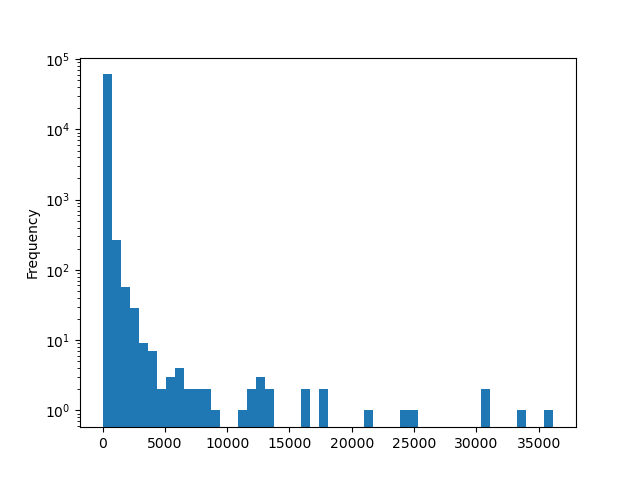
\includegraphics[width=\textwidth]{../experiment/data_analysis/recentCommitCount_distribution}
            \caption{\en{Commits} récents}
        \end{subfigure}
        \begin{subfigure}[t]{0.333\textwidth}
            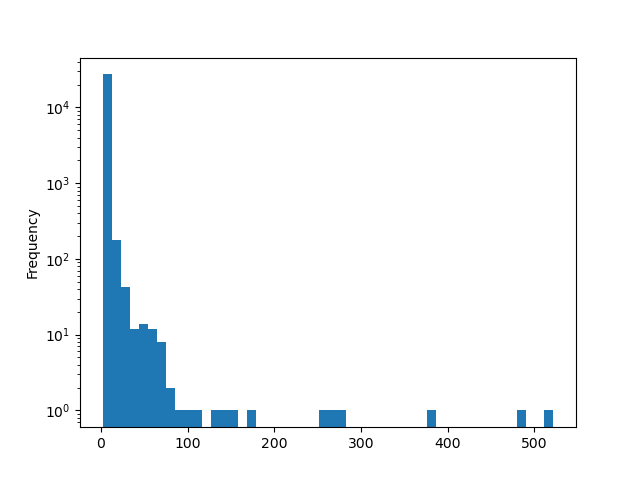
\includegraphics[width=\textwidth]{../experiment/data_analysis/recentContributorCount_distribution}
            \caption{Contributeurs récents}
        \end{subfigure}%
        \begin{subfigure}[t]{0.333\textwidth}
            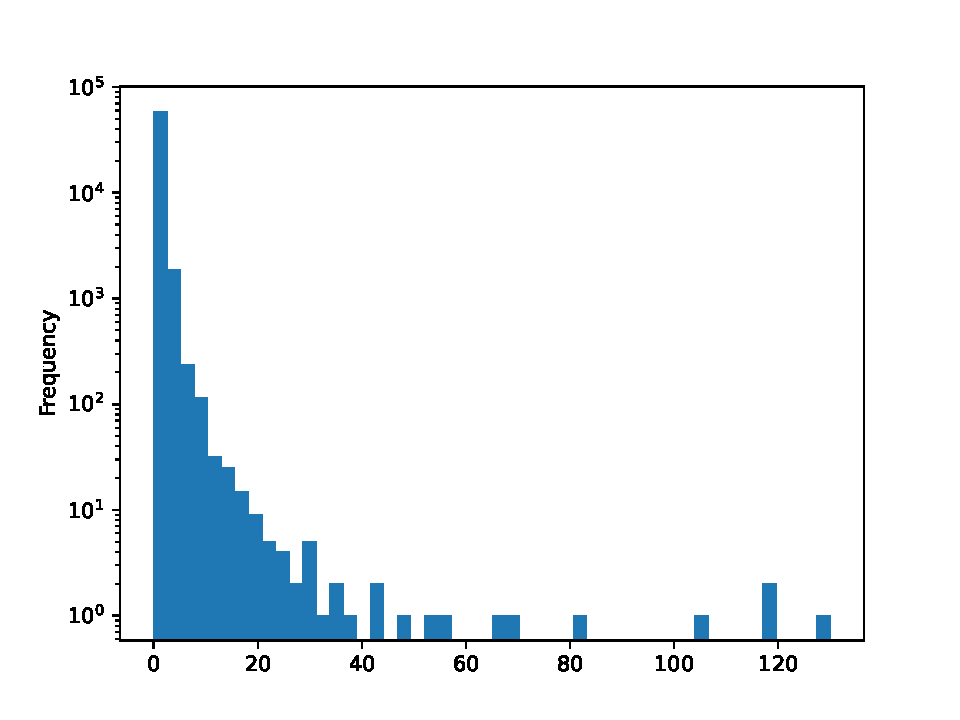
\includegraphics[width=\textwidth]{../experiment/data_analysis/newContributorCount_distribution}
            \caption{Nouveaux contributeurs}
        \end{subfigure}
        \caption{Distributions (avec ordonnée logarithmique) des données étudiées}
        \label{fig:distribution}
    \end{figure}

    Sur les $60 966$ projets distincts (sans historique commun) analysés, $14\%$ d'entre eux possèdent des
    instructions de contribution. Les nombres de \en{commits} récents, de contributeurs récents et de nouveaux
    contributeurs varient fortement au sein de cette population, la distribution n'est normale dans aucun des
    cas (voir Fig.~\ref{fig:distribution}). Les projets possédant des instructions de contribution ont en
    moyenne plus de nouveaux contributeurs (voir Fig.~\ref{fig:hasContrib}) avec une taille d'effet $\rho
    \approx 0.57$ (test MWW), ce qui confirme ($p \approx 0$) que les deux distributions sont bien différentes
    et valide \hyperref[hyp:contributionguidelines]{l'hypothèse H\ref*{hyp:contributionguidelines}}. De
    futures recherches pourraient essayer de déterminer si ce plus grand nombre de nouveaux contributeurs
    \emph{ayant réussi} à contribuer est dû uniquement à ce plus grand nombre de nouveaux contributeurs
    \emph{essayant} de contribuer, ou si la présence d'instructions de contribution a un réel rôle dans le
    succès d'une tentative de contribution. Notons tout de même que la robustesse du test MWW diminue
    significativement dans une situation comme la nôtre (distribution non-normale et variances
    significativement différentes entre les deux catégories) \parencite{WMW-robustness-1998}.

    \begin{figure}
        \centering
        \begin{subfigure}[t]{0.333\textwidth}
            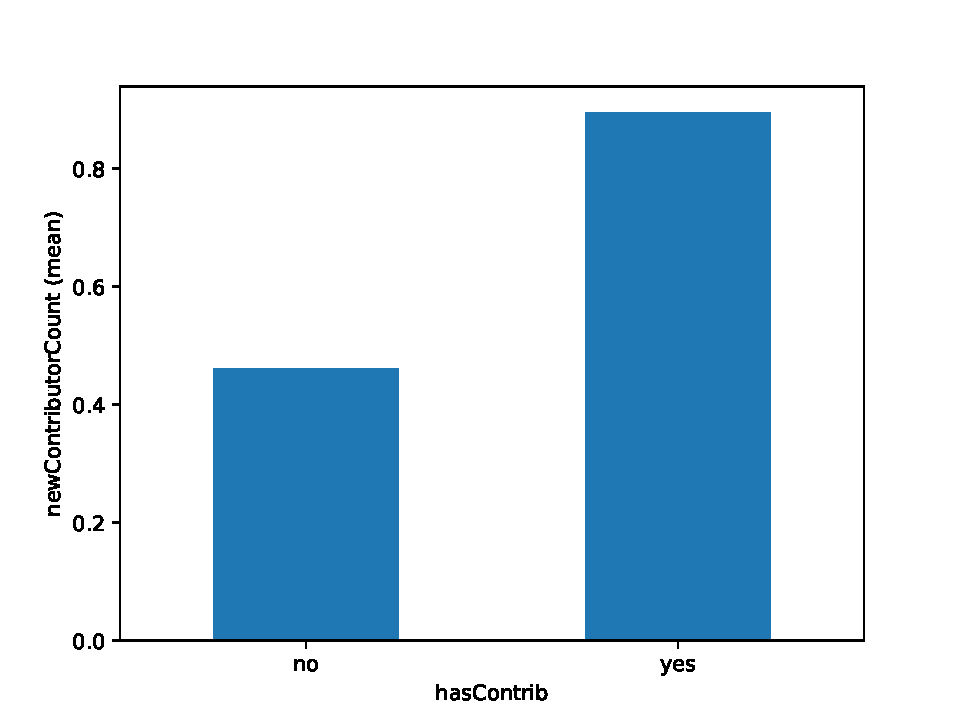
\includegraphics[width=\textwidth]{../experiment/data_analysis/hasContrib_meanNewContributorCount}
            \caption{Présence d'instructions de contribution}
            \label{fig:hasContrib}
        \end{subfigure}%
        \begin{subfigure}[t]{0.333\textwidth}
            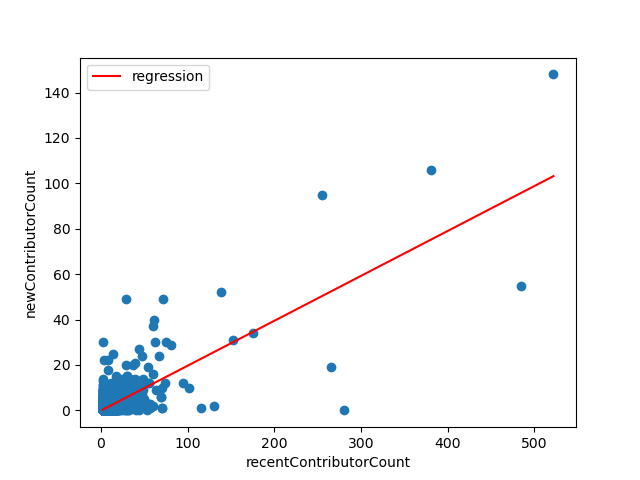
\includegraphics[width=\textwidth]{../experiment/data_analysis/recentContributorCountRegression_linearScale}
            \caption{Nombre de contributeurs récents}
            \label{fig:recentContributors}
        \end{subfigure}%
        \begin{subfigure}[t]{0.333\textwidth}
            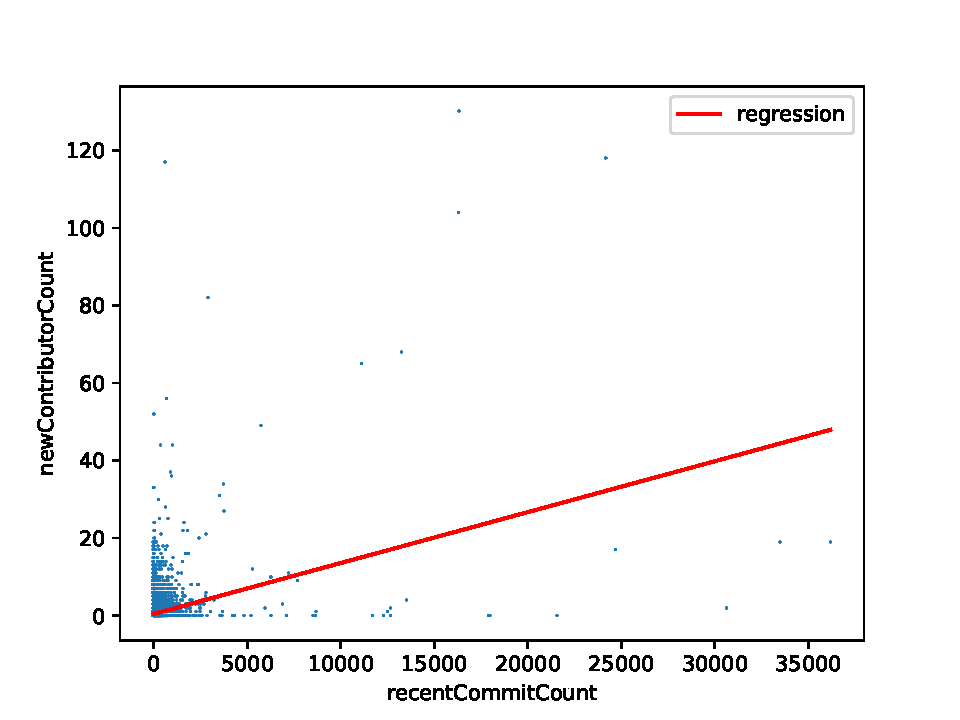
\includegraphics[width=\textwidth]{../experiment/data_analysis/recentCommitCountRegression_linearScale}
            \caption{Nombre de \emph{commits} récents}
            \label{fig:recentCommits}
        \end{subfigure}%

        \caption{Nombre de nouveaux contributeurs en fonction des variables mesurées.}
    \end{figure}

    Une régression
    \href{https://www.statsmodels.org/dev/generated/statsmodels.regression.linear_model.GLS.html}{GLS} suggère
    que plus le nombre de contributeurs récents d'un projet est élevé, plus son nombre de nouveaux
    contributeurs l'est aussi (voir Fig.~\ref{fig:recentContributors}). Le coefficient de détermination $R^2
    \approx 0.45$ du modèle indique que le nombre de contributeurs récents explique environ $45\%$ de la
    variation du nombre de nouveaux contributeurs, ce qui valide
    \hyperref[hyp:recentcontributorcount]{l'hypothèse H\ref*{hyp:recentcontributorcount}}, avec une taille
    d'effet tout de même modérée. Suivant la même approche pour l'analyse du nombre de \en{commits} récents,
    une régression GLS suggère ici aussi une corrélation positive entre le nombre de \en{commits} récents d'un
    projet et son nombre de nouveaux contributeurs (voir Fig.~\ref{fig:recentCommits}), mais son coefficient
    de détermination est trop faible ($R^2 \approx 0.10$) pour considérer que le modèle représente fidèlement
    des données du problème. Nous ne pouvons donc valider \hyperref[hyp:recentcommitcount]{l'hypothèse
    H\ref*{hyp:recentcommitcount}}.

    \section{Conclusion}

    L'analyse de l'archive de Software Heritage nous a permis de trouver une corrélation positive entre le
    nombre de nouveaux contributeurs d'un projet de logiciel libre et deux indicateurs facilement observables
    pour les aspirants contributeurs ou les enseignants souhaitant faire travailler leurs étudiants sur ces
    problématiques : la présence d'instructions de contribution au sein d'un projet et le nombre de
    contributeurs uniques ayant récemment contribué au projet. Nous n'avons en revanche pas trouvé de lien
    avec le nombre de \en{commits} récents des projets. Restent par ailleurs à identifier les liens de
    causalité expliquant nos observations, ainsi que la mise en situation de ces indicateurs dans un contexte
    pédagogique.

    \printbibliography[heading=bibintoc]
\end{document}
